\documentclass[tikz,border=3pt]{standalone}
% Shared preamble for every TikZ figure in the report.
% Colours are Okabe-Ito, with roles fixed across all nine figures.
\usepackage[T1]{fontenc}
\usepackage{lmodern}
\usepackage{amsmath,amssymb}
\usetikzlibrary{arrows.meta,positioning,calc,fit,backgrounds,shapes.geometric,shapes.misc,decorations.pathreplacing,patterns}

\definecolor{cGraph}{HTML}{0072B2}
\definecolor{cSem}{HTML}{E69F00}
\definecolor{cFuse}{HTML}{009E73}
\definecolor{cLoop}{HTML}{D55E00}
\definecolor{cOracle}{HTML}{CC79A7}
\definecolor{cNeutral}{HTML}{999999}
\definecolor{cInk}{HTML}{222222}

\tikzset{
  every picture/.style={line width=0.5pt},
  box/.style={draw=cNeutral!90!black, fill=cNeutral!8, rounded corners=1.6pt,
              align=center, inner sep=3.2pt, font=\small, text=cInk},
  gbox/.style={box, draw=cGraph, fill=cGraph!7},
  sbox/.style={box, draw=cSem!80!black, fill=cSem!12},
  fbox/.style={box, draw=cFuse, fill=cFuse!8},
  lbox/.style={box, draw=cLoop, fill=cLoop!8},
  ann/.style={font=\scriptsize, text=cInk, align=center, inner sep=1.5pt},
  flow/.style={-{Stealth[length=4pt,width=3.2pt]}, draw=cNeutral!85!black},
  gflow/.style={flow, draw=cGraph},
  sflow/.style={flow, draw=cSem!85!black},
}

% Figure labels are short; never hyphenate them.
\hyphenpenalty=10000
\exhyphenpenalty=10000

\begin{document}
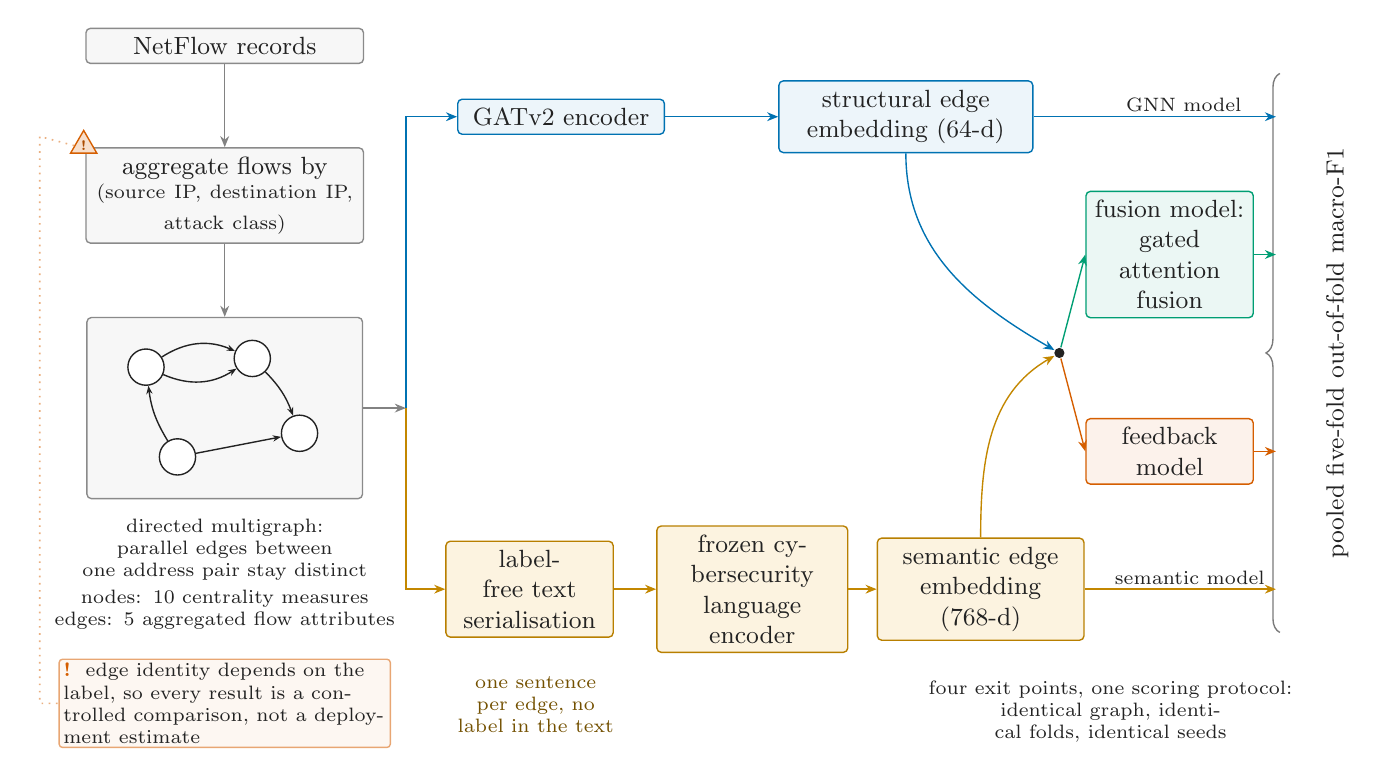
\begin{tikzpicture}[x=1cm,y=1cm]

% ------------------------------------------------------------ shared path
\node[box, text width=3.3cm] (rec) at (1.75,3.9) {NetFlow records};
\node[box, text width=3.3cm] (agg) at (1.75,2.0)
      {aggregate flows by\\[1pt] \scriptsize(source IP, destination IP,\\ attack class)};

\node[box, minimum width=3.5cm, minimum height=2.3cm] (gph) at (1.75,-0.7) {};
\begin{scope}[shift={(1.75,-0.7)}, every node/.style={circle,draw=cInk,fill=white,
              inner sep=0pt,minimum size=4.6mm}]
  \node (n1) at (-1.00, 0.52) {};
  \node (n2) at ( 0.35, 0.63) {};
  \node (n3) at (-0.60,-0.62) {};
  \node (n4) at ( 0.95,-0.32) {};
\end{scope}
\draw[-{Stealth[length=3pt]}, cInk, bend left=28] (n1) to (n2);
\draw[-{Stealth[length=3pt]}, cInk, bend right=28] (n1) to (n2);
\draw[-{Stealth[length=3pt]}, cInk] (n3) to (n4);
\draw[-{Stealth[length=3pt]}, cInk, bend left=12] (n2) to (n4);
\draw[-{Stealth[length=3pt]}, cInk, bend left=12] (n3) to (n1);

\node[ann, anchor=north, text width=4.9cm] (gann) at (1.75,-2.05)
      {directed multigraph: parallel edges between\\ one address pair stay distinct\\[1.5pt]
       nodes: 10 centrality measures\\ edges: 5 aggregated flow attributes};

\draw[flow] (rec) -- (agg);
\draw[flow] (agg) -- (gph);

% the caveat that bounds every claim in the report
\node[regular polygon, regular polygon sides=3, draw=cLoop, fill=cLoop!20,
      inner sep=0.2pt, minimum size=3.4mm, font=\tiny\bfseries, text=cLoop!80!black] (wrn)
      at ($(agg.north west)+(-0.02,0.02)$) {!};
\node[ann, draw=cLoop!55, fill=cLoop!5, rounded corners=1.2pt, text width=4.1cm,
      align=left] (wtxt) at (1.75,-4.45)
      {\textcolor{cLoop}{\bfseries !}\ \ edge identity depends on the label, so every result
       is a controlled comparison, not a deployment estimate};
\draw[cLoop!50, dotted, line width=0.6pt]
      (wrn.west) -- (-0.60,2.75) -- (-0.60,-4.45) -- (wtxt.west);

% ------------------------------------------------------------ the fork
\coordinate (fork) at (4.05,-0.7);
\draw[flow] (gph.east) -- (fork);
\draw[gflow] (fork) |- (4.70,3.0);
\draw[sflow] (fork) |- (4.55,-3.0);

% ------------------------------------------------------------ structural branch
\node[gbox, text width=2.4cm, anchor=west] (gat)  at (4.70,3.0) {GATv2 encoder};
\node[gbox, text width=3.0cm]              (gemb) at (10.40,3.0)
      {structural edge\\ embedding (64-d)};
\draw[gflow] (gat) -- (gemb);

% ------------------------------------------------------------ semantic branch
\node[sbox, text width=1.9cm, anchor=west] (ser) at (4.55,-3.0)
      {label-free text\\ serialisation};
\node[sbox, text width=2.2cm]  (enc)  at (8.45,-3.0)
      {frozen cybersecurity\\ language encoder};
\node[sbox, text width=2.4cm]  (semb) at (11.35,-3.0)
      {semantic edge\\ embedding (768-d)};
\draw[sflow] (ser) -- (enc);
\draw[sflow] (enc) -- (semb);
\node[ann, anchor=north, text=cSem!50!black, text width=2.6cm] at (5.70,-4.05)
      {one sentence per edge, no label in the text};

% ------------------------------------------------------------ where they meet
\node[circle, fill=cInk, inner sep=1.3pt] (jn) at (12.35,0) {};
\draw[gflow] (gemb.south) to[out=-90,in=150] (jn);
\draw[sflow] (semb.north) to[out=90,in=210] (jn);

\node[fbox, text width=1.9cm] (agaf) at (13.75,1.25) {fusion model:\\ gated attention fusion};
\node[lbox, text width=1.9cm] (loop) at (13.75,-1.25) {feedback model};
\draw[flow, draw=cFuse] (jn) -- (agaf.west);
\draw[flow, draw=cLoop] (jn) -- (loop.west);

% ------------------------------------------------------------ one scoring protocol
\draw[decorate, decoration={brace, amplitude=5pt}, draw=cInk!60]
      (15.15,-3.55) -- (15.15,3.55);
\node[rotate=90, font=\small, text=cInk] at (15.88,0)
      {pooled five-fold out-of-fold macro-F1};

\draw[gflow] (gemb.east) -- node[ann, above, pos=0.62]{GNN model} (15.10,3.0);
\draw[sflow] (semb.east) -- node[ann, above, pos=0.55]{semantic model} (15.10,-3.0);
\draw[flow, draw=cFuse] (agaf.east) -- (15.10,1.25);
\draw[flow, draw=cLoop] (loop.east) -- (15.10,-1.25);

\node[ann, anchor=north, text width=5.0cm] at (13.0,-4.10)
      {four exit points, one scoring protocol:\\ identical graph, identical folds, identical seeds};

\end{tikzpicture}
\end{document}
